\documentclass{article}
\usepackage{pgfplots}
\usepackage{filecontents}
\usepackage{tikz}
\usepackage{verbatim}
\pgfplotsset{compat=1.8}
\usepackage{pgfplotstable}

\begin{document}

\newcommand{\scalefactor}{1}
\begin{figure}[t]
  \centering
  \begin{tikzpicture}[scale=\scalefactor, thick]
    \draw[step=0.5cm, gray!50] (-4, -3) grid (4,3); % good idea to have a grid

    \node (A) at (-2.2,-1.8){{\bf A}};
    \node (B) at (2.8,-1.8){{\bf B} = $y_{\bf p}$};

    \node[circle,draw,scale=0.3] (realA) at (2,-1.5) {}; % circle at end of line seg
    \node[circle,draw,scale=0.3] (realB) at (-2,-1.5) {}; % {} no label for circle
    %% \node[circle,draw,scale=0.3] (origin) at (0,0) {};    % just for ref
    \path[draw,very thick] (-2,-1.5) -- (2,-1.5);

    \path[draw, red] (-2, -1) -- (2,2.5);
    \node (cp) at (1, 1.9){${\bf c_p}$};

    %% \draw[dotted]
    %% (0,0) node {1st node}
    %% -- (1,1) node {2nd node}
    %% -- (0,2) node {3rd node}
    %% -- cycle;
    %% \node (x) at (0,0) {x};   % using reference for drawing
    %% \node (y) at (3,1) {y};
    %% \draw (x) -- (y);
    
    \path[draw,blue] (-2, 0) -- (2,1.5);
    \node (cq) at (1,0.8){${\bf c_q}$};

    \path[draw, dotted] (-3,2.5) -- (2,2.5);
    \path[draw, dotted] (-3,-1) -- (-2,-1);
    \path[<->] (-3,-1) edge node[left]{$\delta$} (-3,2.5);

    \path[draw, dotted] (-2.5,0) -- (-2,0);
    \path[<->] (-2.5,0) edge node[right]{$\Delta$} (-2.5,-1);

    \path[draw, dotted] (-2.5,1.5) -- (2,1.5);
    \path[<->] (-2.5,1.5) edge node[right, align=center]{\small decrease in \\ \small value of ${\bf y_p}$}(-2.5,2.5);

    \path[->, dashed, sloped] (-3.5,-3) edge node[above]{\small increasing objective}  (-3.5,3);

    \node (maxC) at (2.8,2.5) {${\bf c_{\bf p}}^T{y_{\bf p}}$};

    \node at (0,-2.5){\small Two assignments};
    \path[draw,->, dotted] (1.1,-2.4) -- (B);
    \path[draw,->, dotted] (-1.1,-2.35) -- (A);

  \end{tikzpicture}
  \caption{{\footnotesize An illustration of the margin-based
      amortization scheme showing the very simple case with only two
      competing assignments {\bf A} and {\bf B}.}}
  \label{fig:theorem-figure}
\end{figure}

%%%%%%%%%%%%%%%%%%%%%%%%%%%%%%
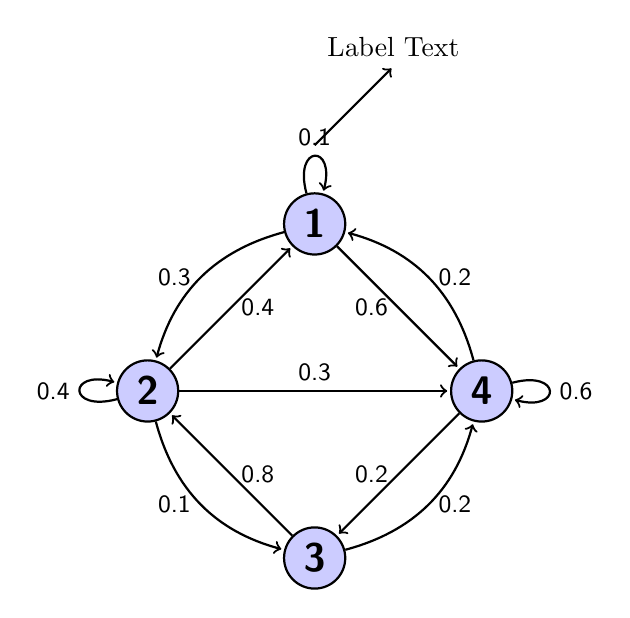
\begin{tikzpicture}[->,shorten >=1pt,auto,node distance=3cm,
    thick,main node/.style={circle,fill=blue!20,draw,font=\sffamily\Large\bfseries}]
  \draw (0,1) -- (1,2) node [above, fill=white] {Label Text};
  \node[main node] (1) {1};
  \node[main node] (2) [below left of=1] {2};
  \node[main node] (3) [below right of=2] {3};
  \node[main node] (4) [below right of=1] {4};

  \path[every node/.style={font=\sffamily\small}]
  (1) edge node [left] {0.6} (4)
  edge [bend right] node[left] {0.3} (2)
  edge [loop above] node {0.1} (1)
  (2) edge node [right] {0.4} (1)
  edge node {0.3} (4)
  edge [loop left] node {0.4} (2)
  edge [bend right] node[left] {0.1} (3)
  (3) edge node [right] {0.8} (2)
  edge [bend right] node[right] {0.2} (4)
  (4) edge node [left] {0.2} (3)
  edge [loop right] node {0.6} (4)
  edge [bend right] node[right] {0.2} (1);
\end{tikzpicture}

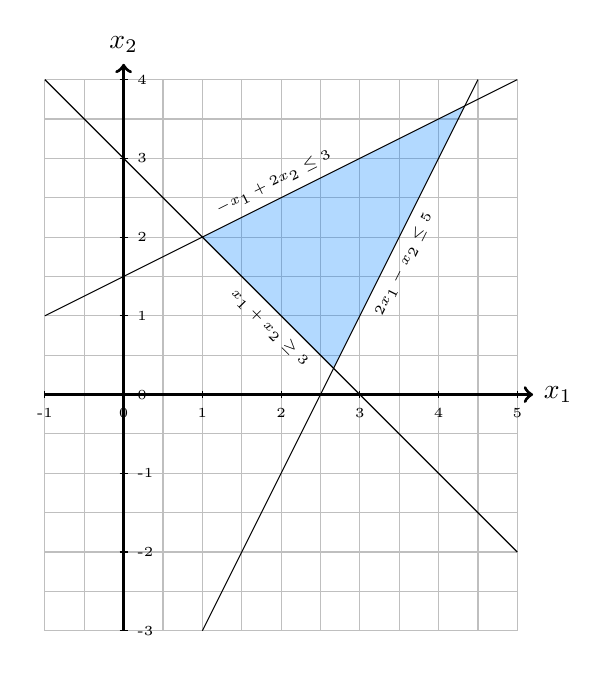
\begin{tikzpicture}
  \draw[gray!50, thin, step=0.5] (-1,-3) grid (5,4);
  \draw[very thick,->] (-1,0) -- (5.2,0) node[right] {$x_1$};
  \draw[very thick,->] (0,-3) -- (0,4.2) node[above] {$x_2$};
  \foreach \x in {-1,...,5} \draw (\x,0.05) -- (\x,-0.05) node[below] {\tiny\x};
  \foreach \y in {-3,...,4} \draw (-0.05,\y) -- (0.05,\y) node[right] {\tiny\y};
  \fill[blue!50!cyan,opacity=0.3] (8/3,1/3) -- (1,2) -- (13/3,11/3) -- cycle;
  \draw (-1,4) -- node[below,sloped] {\tiny$x_1+x_2\geq3$} (5,-2);
  \draw (1,-3) -- (3,1) -- node[below left,sloped] {\tiny$2x_1-x_2\leq5$} (4.5,4);
  \draw (-1,1) -- node[above,sloped] {\tiny$-x_1+2x_2\leq3$} (5,4);
\end{tikzpicture}

%% this will generate gnuplot scripts, you have to run them to generate the data to be plotted.
%% \begin{tikzpicture}[domain=0:4]
%%   \draw[very thin,color=gray] (-0.1,-1.1) grid (3.9,3.9);
%%   \draw[->] (-0.2,0) -- (4.2,0) node[right] {$x$};
%%   \draw[->] (0,-1.2) -- (0,4.2) node[above] {$f(x)$};
%%   \draw[color=red] plot[id=x] function{x}
%%   node[right] {$f(x) =x$};
%%   \draw[color=blue] plot[id=sin] function{sin(x)}
%%   node[right] {$f(x) = \sin x$};
%%   \draw[color=orange] plot[id=exp] function{0.05*exp(x)}
%%   node[right] {$f(x) = \frac{1}{20} \mathrm e^x$};
%% \end{tikzpicture}

\end{document}
